\section{任务2\quad 图像异常检测}
\label{sec:task2}
\subsection{问题描述与定义}
当产品类别 $c\in\{\text{hazelnut},\text{zipper}\}$ 已知时，给定该类训练集 $\mathcal D_c=\{(x_i,y_i)\}$，其中 $y=0$ 表示正常，$y=1$ 表示异常。目标是为待测图像 $x$ 学习异常分数 $s_c(x)$，分数越大越倾向于异常。按 $\widehat y=\mathbf 1[s_c(x)\ge t_c]$ 产生图像级判定，其中 $t_c$ 由训练集确定。训练中正常与异常样本之比为 $4:1$，分别按产品训练。该任务的标签是图像级，局部热图仅用于观察模型响应。

\begin{table}[H]
 \caption{异常检测数据划分}
 \label{tab:anomaly-data}
 \centering
 \begin{tabular}{@{}lrrrr@{}}
 \toprule
 产品 & 训练正常 & 训练异常 & 测试正常 & 测试异常 \\
 \midrule
 榛子 & 200 & 50 & 40 & 15 \\
 拉链 & 200 & 50 & 32 & 15 \\
 \bottomrule
 \end{tabular}
\end{table}

训练沿用课程划分（表\ref{tab:anomaly-data}）。公开 MVTec AD 提供了工业外观检测的实验背景\cite{bergmann2019}，本报告的结果对应课程发放的类别、样本与划分。测试集标签在模型、阈值和逐图分数固定后用于计分。

\subsection{图像特征表示}
榛子的小孔和拉链的不连续均可能只占很小面积。将原图双线性缩放至 $384\times384$，保持 RGB 通道和整幅视野。沿用任务1的 ImageNet 通道归一化和冻结网络。对整图分支，以 \texttt{layer2} 和 \texttt{layer3} 的通道均值及标准差、\texttt{layer4} 的通道均值、以及颜色块表示图像。按任务1的方法做开平方、分块归一化与加权拼接，六个权重依次为 $0.18,\allowbreak 0.12,\allowbreak 0.22,\allowbreak 0.13,\allowbreak 0.25,\allowbreak 0.10$，特征总维数为 5\,360。

对局部分支，从网络的前三层残差阶段取特征图。先做 $3\times3$ 局部均值池化，再对齐到 $24\times24$ 网格。每层、每位置的通道向量分别作 $\ell_2$ 归一化。将浅中层（第1、2阶段）和中层（第2、3阶段）分别拼接成两套图像块特征。各用固定种子的高斯随机矩阵投影为 48 维，再做 $\ell_2$ 归一化，以降低正常图像块检索的内存和计算开销。浅层保留相邻纹理和边缘，中层覆盖更大感受野。

\begin{figure*}[t]
 \centering
 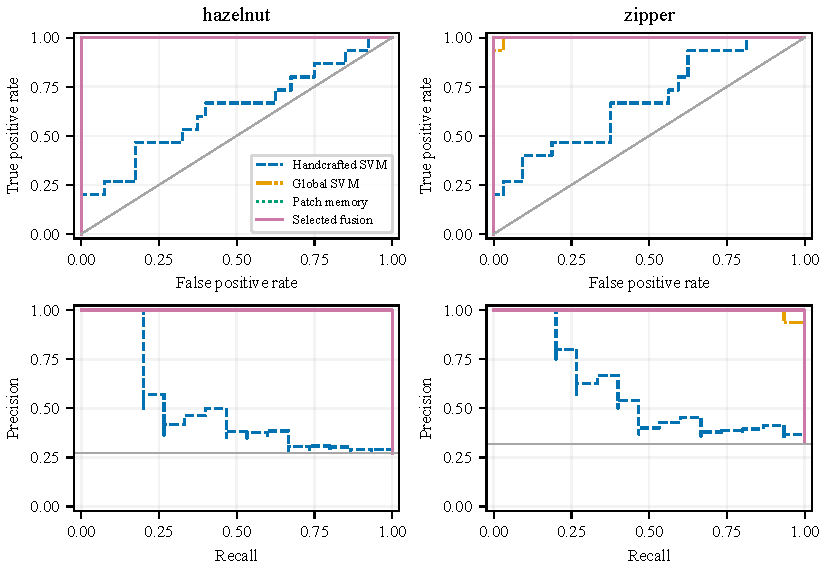
\includegraphics[width=.73\textwidth]{anomaly_curves}
 \caption{测试集的 ROC 和 PR 曲线。PR 图的灰线表示各产品的异常样本比例}
 \Description{The patch and fusion curves overlap at perfect ranking for both products. The handcrafted baseline ranks samples substantially less accurately.}
 \label{fig:anomaly-curves}
\end{figure*}

\subsection{方法}
\textbf{正常图像块最近邻。} 借鉴 PatchCore 的正常图像块记忆库思想\cite{roth2022}。每张训练正常图在每套特征上均匀无放回抽取 64 个位置。记某套训练记忆库为 $B$，查询位置 $u$ 的归一化向量为 $\vect p_u$，其局部分数为
\begin{equation}
 d_u=1-\max_{\vect b\in B}\vect p_u^\top\vect b.
\end{equation}
对 $24\times24$ 网格中的分数排序，取最大的 $\lceil q\cdot576\rceil$ 个求均值。比起对全图平均，只聚合尾部可以保留范围很小的缺陷。两套特征的图像级分数先按训练集折外正常分数的中位数和四分位距进行标准化，再取均值，得到 $s_{\mathrm p}$。局部模型只用正常图构建记忆库，训练异常图用于选择聚合比例。

\textbf{整图分类器。} 用训练集中有标签的正常图和异常图训练径向基核 SVM，采用
$k(\vect z_i,\vect z_j)=\exp(-\gamma\|\vect z_i-\vect z_j\|_2^2)$。
异常类权重为正常类的四倍，以抵消训练样本数量差异。记有符号决策分数为 $s_{\mathrm g}$，正方向对应异常。整图分类器可学习训练集中典型的缺陷响应，正常库分支则反映图像块和已见正常模式的偏离程度。

\textbf{融合与阈值。} 每类做五折分层验证。每折训练使用 160 张正常图与 40 张异常图，验证使用其余 40 张正常图和 10 张异常图。每折每套正常库有 10\,240 个图像块。折外分数来自未使用该训练样本的模型。令 $R(s)=(s-m)/\max(r,10^{-8})$ 表示按正常折外分数的中位数 $m$ 和四分位距 $r$ 缩放。融合分数为
\begin{equation}
 s_c(x)=wR_{\mathrm p}(s_{\mathrm p}(x))+(1-w)R_{\mathrm g}(s_{\mathrm g}(x)).
\end{equation}
候选聚合比例 $q$ 为 1\%、5\% 和 15\%。SVM 的 $C$ 从 $\{0.5,2,8,32\}$ 选择，$\gamma$ 从 $\{0.25,1,4\}$ 选择。融合权重 $w$ 从 0 到 1，以 0.25 为步长枚举。各阶段先比较折均 AUROC，同分时比较折均 AP。最终汇总训练折外分数，选取最大化 $\mathrm{TPR}-\mathrm{FPR}$ 的阈值，同分时用较低阈值。对测试图，分别运行五个折模型并平均各分支分数，使用固定的融合权重和阈值判断。

\begin{table}[tbp]
 \caption{训练集选出的异常检测参数}
 \label{tab:anomaly-parameters}
 \centering
 \begin{tabular}{@{}lrrrrrr@{}}
 \toprule
 产品 & $q$ & $C$ & $\gamma$ & $w$ & $t_c$ & 折均 AUROC \\
 \midrule
 榛子 & 1\% & 8 & 4 & 0.50 & 1.6771 & 1.0000 \\
 拉链 & 15\% & 32 & 4 & 0.50 & 1.4314 & 0.9995 \\
 \bottomrule
 \end{tabular}
\end{table}

表\ref{tab:anomaly-parameters}显示，榛子采用最高的 6 个响应，拉链采用最高的 87 个响应。前者聚焦小面积的强响应，后者汇总更宽范围内的局部变化。训练折参与模型选择，独立测试集用于估计最终效果。若记每套记忆库大小为 $M$，位置数为 $P$，投影维数为 $d$，单次最近邻打分用时 $O(PMd)$，实现分批取最大相似度。

\begin{figure*}[t]
 \centering
 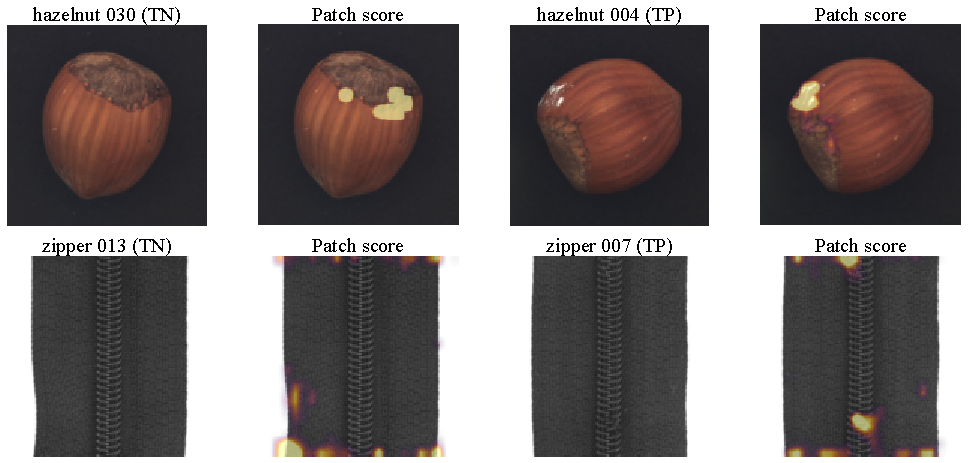
\includegraphics[width=.85\textwidth]{anomaly_examples}
 \caption{各产品距阈值最近的正常图和异常图。热图高亮局部近邻距离较大的区域}
 \Description{Original images and patch-score overlays for hazelnut 030 and 004, and zipper 013 and 007.}
 \label{fig:anomaly-examples}
\end{figure*}

\subsection{实验结果分析}
将异常视为正类。AUROC 衡量异常样本排在正常样本前面的能力，AP 按召回的增量加权各点精确率。固定阈值后报告准确率、精确率、召回率及其调和平均 F1。宏平均是两类指标的等权平均。手工对照使用颜色和灰度差分特征，固定 $C=2$、$\gamma=1$。整图 SVM 和正常图像块模型单独运行，采用各自的训练折外阈值。

\begin{table}[tbp]
 \caption{独立测试集上的异常检测对照}
 \label{tab:anomaly-results}
 \centering
 \begin{tabular}{@{}llrrrr@{}}
 \toprule
 产品 & 方法 & AUROC & AP & ACC & F1 \\
 \midrule
 榛子 & 手工 SVM & .632 & .506 & .291 & .435 \\
      & 整图 SVM & 1.000 & 1.000 & 1.000 & 1.000 \\
      & 正常块近邻 & 1.000 & 1.000 & 1.000 & 1.000 \\
      & 融合 & 1.000 & 1.000 & 1.000 & 1.000 \\
 \addlinespace
 拉链 & 手工 SVM & .683 & .590 & .532 & .500 \\
      & 整图 SVM & .998 & .996 & .979 & .968 \\
      & 正常块近邻 & 1.000 & 1.000 & 1.000 & 1.000 \\
      & 融合 & 1.000 & 1.000 & 1.000 & 1.000 \\
 \addlinespace
 宏平均 & 手工 SVM & .658 & .548 & .411 & .467 \\
      & 整图 SVM & .999 & .998 & .989 & .984 \\
      & 正常块近邻 & 1.000 & 1.000 & 1.000 & 1.000 \\
      & 融合 & 1.000 & 1.000 & 1.000 & 1.000 \\
 \bottomrule
 \end{tabular}
\end{table}

融合模型的混淆计数 $(\mathrm{TN},\mathrm{FP},\mathrm{FN},\mathrm{TP})$ 在榛子上为 $(40,0,0,15)$，在拉链上为 $(32,0,0,15)$，两类精确率与召回率均为 1.000。手工特征丢失了具体缺陷的位置，测试中误报明显增加。拉链的整图模型把正常图 \texttt{032.png} 判为异常，局部模型和融合模型均判为正常。榛子测试集中最高的正常分数为 1.209、最低的异常分数为 2.808，拉链对应为 1.307 和 2.218，两类的训练阈值均位于相应间隔内。融合比两个单分支在训练折上的排序表现略好，与局部模型在独立测试集上并列。曲线重叠见图\ref{fig:anomaly-curves}。

图\ref{fig:anomaly-examples}展示正常与异常图各自最接近阈值的样本。榛子异常图的高响应集中在可见缺陷附近，拉链正常图的边缘也有较强响应。热图在各图内单独归一化，图像间的分数比较使用模型原始输出。测试集中每类只有 15 张异常图。按同一产品内独立同分布的二项模型估计，两类准确率的 95\% Clopper--Pearson 区间分别为 $[0.935,1.000]$ 和 $[0.925,1.000]$。由于当前测试集不存在正负排序颠倒，经验重采样会给出退化的 AUROC 区间，无法反映新批次的不确定性。测试结果覆盖现有产品和成像条件，仍需在新的缺陷类型和光照下复核。

